%\documentclass[oldversion,referee]{aa}
\documentclass[]{aa}
%\documentclass[]{aa}
\usepackage{graphicx}
\usepackage{psfig}
\usepackage{epstopdf}
\usepackage{amssymb}
\usepackage{amsmath}
\usepackage{verbatim}
\usepackage{natbib}
\usepackage{rotate}
\usepackage{lscape}
%\usepackage{dsfont}
\usepackage{aalongtable}
\usepackage{supertabular}
\usepackage{mathbbol}
\usepackage{bm}
\usepackage{mathtools}
%\usepackage[subnum]{cases}
\usepackage{enumerate}
%\usepackage{draftcopy}
%\psdraft
%\usepackage[sc]{titlesec}
%\usepackage{bold-extra}
\usepackage{arydshln}
\usepackage{amsmath}

\bibpunct{(}{)}{;}{a}{}{,}

\newcommand{\tbsp}{\rule{0pt}{18pt}}
\newcommand\sqdeg{deg$^{2}$}
\newcommand\psqdeg{deg$^{-2}$}
\newcommand\ugriz{u$^*$g'r'i'z'}
\newcommand\mic{$\mu$m}
\newcommand\AAn{\AA~}
\newcommand\sfr{SFR$_{0.5}$}
\newcommand\ssfr{sSFR$_{0.5}$}
\newcommand\msol{\mbox{M$_{\odot}$}}
\newcommand\wph{W.Hz$^{-1}$}
\newcommand\lsol{\mbox{L$_{\odot}$}}
\newcommand{\appropto}{\mathrel{\vcenter{
  \offinterlineskip\halign{\hfil$##$\cr
    \propto\cr\noalign{\kern2pt}\sim\cr\noalign{\kern-2pt}}}}}
%\usepackage{newtxtext,newtxmath}

\def\mathY{\bm{\mathcal{Y}}}
%\def\mathY{\bm{\mathcal{V}}}
\def\Bchi{\large\bm{\mathcal{\chi}}}
%\def\Bchi{\chi}
\def\PVec{\textbf{x}}
%% ======= Names   =====================
\def\COH{{\sc CohJones}}

% ======= Scalars =====================
\def\u{u}
\def\v{v}
\def\w{w}
\def\l{l}
\def\m{m}
\def\n{n}
%\def\d{\text{d}}
\def\d{d}
\def\dbf{{\bm d}}


% ======= Conjugates
%\newcommand{\conj}[1]{{#1}^*}
%\newcommand{\conjp}[1]{{\left(#1\right)}^*}
\newcommand{\conj}[1]{\overline{#1}}
\newcommand{\conjp}[1]{\left({\overline{#1}}\right)}


% ======= 2x2 Matrices ===============
\def\JMat{\textbf{J}}
\def\Skyd{\textbf{S}_d}
\def\Vbl{\textbf{V}_{(pq)t\nu}}

\newcommand{\mat}[1]{{\bm{#1}}}
\newcommand{\JJ}{\mat{J}} % \bmath{\mathcal{J}}}
\newcommand{\JHJ}{\JJ^H\JJ} % \bmath{\mathcal{J}}}

% ======= Vectors      ===============
\def\vbltnu{\textbf{v}_{(pq)t\nu}}
\def\vbl{\textbf{v}_{pq}}
\def\V{\textbf{V}}
\def\gwirt{\bm{g_{\!_{W}}}}
\def\dgwirt{\dbf\bm{g_{\!_{W}}}}
\def\g{\bm{g}}
\def\vis{\textbf{v}}

% ====== Separator    ================
\def\separator{
\hrule
\begin{center}
\textsc{to be modified after that}
\end{center}
\hrule
}

% ======= Kroneker product ===========
\def\Kron{\otimes}

% ======= Jacobians =====================
\def\SimpleJacob{\bm{J}}
\def\Jacob{\bm{\mathcal{J}}}
%\def\JVpq{\Jacob\left\{\textbf{v}_{(pq)}\right\}}
%\def\JVpq{\Jacob_{\!_{\textbf{v}_{pq}}}}
\def\JVpq{\Jacob_{{\textbf{v}_{pq}},\bm{g_{\!_{W}}}}}
%\def\JVpq{\Jacob_{{\textbf{v}_{pq}}}}

\def\JVpqg{\Jacob_{{\textbf{v}_{pq}},\bm{g}}}
\def\JVpqCg{\Jacob_{{\textbf{v}_{pq}},\bm{\conj{g}}}}
%\def\JVpqg{\Jacob_{{\textbf{v}_{pq}}}\big|_{\bm{g}}}
%\def\JVpqCg{\Jacob_{{\textbf{v}_{pq}}}\big|_{\bm{\conj{g}}}}
\def\JVAtg{\JV\big|_{\vec{g}}}

\def\A{\textbf{A}}
\def\H{\textbf{H}}

\def\JV{\Jacob\left\{\textbf{v}\right\}}
%\def\JV{\Jacob_{\!_\textbf{v}}}
\def\JV{\Jacob_{\textbf{v}}}
%\def\JVpq{\Jacob_{\textbf{V}_{(pq)}}}
\def\JVg{\Jacob_{\textbf{v},\bm{g}}}
\def\JVCg{\Jacob_{\textbf{v},\bm{\conj{g}}}}

\newcommand{\FigDir}{../Figures/}


 \def\supertiny{ \font\supertinyfont = cmr10 at 4pt \relax \supertinyfont}



\begin{document}      

\title{\vspace{-5cm}\\
Applying Wirtinger derivatives to the radio interferometry calibration problem}

\subtitle{}
\author{C. Tasse\inst{1,2}}

\institute{
GEPI, Observatoire de Paris, CNRS, Universit\'e Paris Diderot,
5 place Jules Janssen, 92190 Meudon, France
\and
Department of Physics \& Electronics, Rhodes University, PO Box 94,
Grahamstown, 6140, South Africa
}
%   \author{}
%   \offprints{}
%   \institute{}
%\date{}%Received <date> / Accepted <date>}


\abstract{This paper presents a fast algorithm for full-polarisation,
  direction dependent calibration in radio interferometry. It is based
  on Wirtinger's approach to complex differentiation. Compared to the
  classical case, the Jacobian
  appearing in the Levenberg-Maquardt iterative scheme presents a
  sparser structure, allowing for an significant algorithmic cost gain.
  %corresponding to the number of antenna squared. 
  %This improvement is
  %significant and
  %varies between $\sim10^3$ for VLA or LOFAR to $\sim10^{6-7}$ for the SKA. 
}

\authorrunning{C. Tasse}



%% \authorrunning{}
\titlerunning{Applying Wirtinger derivatives to the radio interferometry calibration problem}
   \maketitle

% ======= Names   =====================
\def\COH{{\sc CohJones}}

% ======= Scalars =====================
\def\u{u}
\def\v{v}
\def\w{w}
\def\l{l}
\def\m{m}
\def\n{n}
%\def\d{\text{d}}
\def\d{d}
\def\dbf{{\bm d}}


% ======= Conjugates
%\newcommand{\conj}[1]{{#1}^*}
%\newcommand{\conjp}[1]{{\left(#1\right)}^*}
\newcommand{\conj}[1]{\overline{#1}}
\newcommand{\conjp}[1]{\left({\overline{#1}}\right)}


% ======= 2x2 Matrices ===============
\def\JMat{\textbf{J}}
\def\Skyd{\textbf{S}_d}
\def\Vbl{\textbf{V}_{(pq)t\nu}}

\newcommand{\mat}[1]{{\bm{#1}}}
\newcommand{\JJ}{\mat{J}} % \bmath{\mathcal{J}}}
\newcommand{\JHJ}{\JJ^H\JJ} % \bmath{\mathcal{J}}}

% ======= Vectors      ===============
\def\vbltnu{\textbf{v}_{(pq)t\nu}}
\def\vbl{\textbf{v}_{pq}}
\def\V{\textbf{V}}
\def\gwirt{\bm{g_{\!_{W}}}}
\def\dgwirt{\dbf\bm{g_{\!_{W}}}}
\def\g{\bm{g}}
\def\vis{\textbf{v}}

% ====== Separator    ================
\def\separator{
\hrule
\begin{center}
\textsc{to be modified after that}
\end{center}
\hrule
}

% ======= Kroneker product ===========
\def\Kron{\otimes}

% ======= Jacobians =====================
\def\SimpleJacob{\bm{J}}
\def\Jacob{\bm{\mathcal{J}}}
%\def\JVpq{\Jacob\left\{\textbf{v}_{(pq)}\right\}}
%\def\JVpq{\Jacob_{\!_{\textbf{v}_{pq}}}}
\def\JVpq{\Jacob_{{\textbf{v}_{pq}},\bm{g_{\!_{W}}}}}
%\def\JVpq{\Jacob_{{\textbf{v}_{pq}}}}

\def\JVpqg{\Jacob_{{\textbf{v}_{pq}},\bm{g}}}
\def\JVpqCg{\Jacob_{{\textbf{v}_{pq}},\bm{\conj{g}}}}
%\def\JVpqg{\Jacob_{{\textbf{v}_{pq}}}\big|_{\bm{g}}}
%\def\JVpqCg{\Jacob_{{\textbf{v}_{pq}}}\big|_{\bm{\conj{g}}}}
\def\JVAtg{\JV\big|_{\vec{g}}}

\def\A{\textbf{A}}
\def\H{\textbf{H}}

\def\JV{\Jacob\left\{\textbf{v}\right\}}
%\def\JV{\Jacob_{\!_\textbf{v}}}
\def\JV{\Jacob_{\textbf{v}}}
%\def\JVpq{\Jacob_{\textbf{V}_{(pq)}}}
\def\JVg{\Jacob_{\textbf{v},\bm{g}}}
\def\JVCg{\Jacob_{\textbf{v},\bm{\conj{g}}}}




%===============================
\section{Complex optimisation}
\label{sec:Wirtinger}

Given a set of cross correlations between antenna voltages (the
visibility set) in a given time-frequency domain and a model of the sky brightness, the calibration
step in radio interferometry consists in estimating a set of
direction-dependent Jones matrices per antenna. This is usually done
using a chi-square minimisation technique such as the
Levenberg-Maquardt. In this paper, I use the alternative Wirtinger's
definition of complex derivative, instead of what is usually done by
considering the real and imaginary (later referred as the
{\it Wirtinger} and {\it classical} approaches respectively).

\subsection{RIME formalism}

Using the Radio Interferometry Measurement Equation (RIME) formalism
\citep[][]{Hamaker96}, the
4-polarisation visibility vector $\vbl$ measured on baseline $(pq)$,
at time $t$ and frequency $\nu$ can be written as


\begin{alignat}{2}
\label{eq:ME}
\vbl=&\text{Vec}\left(\Vbl\right)&\\
=&\displaystyle\sum\limits_{d} \left(\conj{\JMat^{d}_{qt\nu}}\Kron \JMat^{d}_{pt\nu}\right)
\text{Vec}\left(\Skyd\right) k^{d}_{(pq)t\nu}\\
\text{with}\ k^{d}_{(pq)t\nu}=&\exp{\left(-2 i\pi
  \left(\u\l+\v\m+\w\left(\text{n}-1\right)\right)\right)}\\
\text{and}\ \n=&\sqrt{1-\l^2-\m^2}
\end{alignat}

\noindent where $\JMat^{d}_{pt\nu}$ is the Jones matrix of antenna $p$
in direction $d$, $\Skyd$ is the four-polarization sky matrix, $\Kron$
is the Kronecker product, $[\u,\v,\w]^T$ is the baseline vector between antennas
$p$ and $q$ in wavelength units, and
$\vec{s}_d=[\l,\m,\n=\sqrt{1-\l^2-\m^2}]^T$ is a sky direction later
labeled as $d$.
In the following, the Jones matrix $\JMat^{d}_{pt\nu}$ is
represented by scalars $g^{d}_{pt\nu,k}$ as

\begin{equation}
\JMat^{d}_{pt\nu}=
\begin{bmatrix}
g^{d}_{pt\nu,0} & g^{d}_{pt\nu,2} \\ 
g^{d}_{pt\nu,1} & g^{d}_{pt\nu,3} 
\end{bmatrix}
\end{equation}

\noindent and the set of Jones matrices is represented by a gain
vector $\vec{g}$ containing the scalars $g^{d}_{pt\nu,k}$ for all
directions, antennas and polarisations.

From Eq. \ref{eq:ME}, the $i^{th}$ polarisation component of $\vbl$
can be written as

\begin{alignat}{2}
\label{eq:hpq}
\mathrm{v}^i_{pqt\nu}=&h^i_{pq}(\vec{g})\\
=&
\displaystyle\sum\limits_{d}
\displaystyle\sum\limits_{j=0}^3 \left(g^{d}_{pt\nu,\textbf{A}_{ij}}.\conj{g^{d}_{qt\nu,\textbf{B}_{ij}}}\right).k^{d}_{pqt\nu}.\text{s}_{d,j}
\end{alignat}

\noindent where 

\begin{equation}
\textbf{A}=
\begin{bmatrix}
0 & 2 & 0 & 2 \\ 
1 & 3 & 1 & 3 \\ 
0 & 2 & 0 & 2 \\
1 & 3 & 1 & 3 
\end{bmatrix}
\text{ and }
\textbf{B}=
\begin{bmatrix}
0 & 0 & 2 & 2 \\ 
0 & 0 & 2 & 2 \\ 
1 & 1 & 3 & 3 \\
1 & 1 & 3 & 3 
\end{bmatrix}
\end{equation}



\subsection{Wirtinger complex derivative}
\label{sec:Cderiv}

In order to compute a Jacobian, a
derivative definition for complex numbers has to be chosen. Instead of
differentiating against real and imaginary parts independently, one can
adopt a Wirtinger differentiation point of view and consider the
complex and their conjugate as being independent. Choosing this type of differentiation
turns out to be rather powerful to solve problems of the form of
Eq. \ref{eq:ME} (see
Sec. \ref{sec:Solver}). If a complex number is written as $z=x+iy$, the
Wirtinger complex derivative operator becomes


\begin{alignat}{3}
\frac{\partial }{\partial z}&=&\frac{1}{2}\left(\frac{\partial }{\partial x}-i\frac{\partial }{\partial y}\right)\\
\text{and }\frac{\partial }{\partial \conj{z}}&=&\frac{1}{2}\left(\frac{\partial }{\partial x}+i\frac{\partial }{\partial y}\right)
\end{alignat}

\noindent where $x$ and $y$ are the real and imaginary parts
respectively. The
Wirtinger has a trivial but remarkable property that a scalar and its
complex conjugate can be viewed as independent variables, and in
particular

%% \begin{alignat}{3}
%% \label{eq:propConj}
%% \frac{\partial \conj{z}}{\partial z}&=&0
%% \end{alignat}

\begin{equation}
\label{eq:propConj}
\frac{\partial \conj{z}}{\partial z}=0
\text{ and }
\frac{\partial z}{\partial \conj{z}}=0
\end{equation}


Considering the sky, gain, and geometry relation given in
Eq. \ref{eq:ME}, according to the property of Wirtinger derivative of complex
conjugate (Eq. \ref{eq:propConj})

\begin{alignat}{3}
\label{eq:Deriv_gp}
\frac{\partial \mathrm{v}^i_{pqt\nu}}{\partial g^{d}_{pt\nu,\textbf{A}_{ij}}}=&
\left(\conj{g^{d}_{qt\nu,\textbf{B}_{ij}}}\text{s}_{d,j}\right).k^{d}_{pqt\nu}\\
\label{eq:Deriv_gq}
\text{and}\ 
\frac{\partial \mathrm{v}^i_{pqt\nu}}{\partial g^{d}_{qt\nu,\textbf{B}_{ij}}}=&0
\end{alignat}

\noindent while differentiating against the complex conjugate of those
variables, one obtain

\begin{alignat}{3}
\label{eq:Deriv_Cgp}
\frac{\partial \mathrm{v}^i_{pqt\nu}}{\partial \conjp{g^{d}_{pt\nu,\textbf{A}_{ij}}}}=&0\\
\label{eq:Deriv_Cgq}
\text{and}\ 
\frac{\partial \mathrm{v}^i_{pqt\nu}}{\partial \conjp{g^{d}_{qt\nu,\textbf{B}_{ij}}}}=&
\left(g^{d}_{pt\nu,\textbf{A}_{ij}}\text{s}_{d,j}\right).k^{d}_{pqt\nu}
\end{alignat}

Interestingly, Eq. \ref{eq:Deriv_gp},
\ref{eq:Deriv_gq}, \ref{eq:Deriv_Cgp} and \ref{eq:Deriv_Cgq} show that the
derivatives are always constant with respect to the differential
variable.

\subsection{Wirtinger Jacobian}
\label{sec:WirtingerJacob}

This section describes the structure of the Wirtinger Jacobian $\JV$ using the
results of Sec. \ref{sec:Cderiv}.
First, let consider the visibility vector $\vbl$
for all given time frequency blocks, and write the antenna,
polarisation, and direction dependent gain vector as
$\vec{g}$. Its size is $4n_an_d$, and have for $k^{th}$ component
$k=j+4\times d+4\times a \times n_d$ the gain of antenna $a$ in
direction $d$ for polarisation $j$, where $n_a$, and $n_d$ are the
number of antenna and directions.

The corresponding Wirtinger Jacobian $\JVpq$ has size $(4n_t n_{\nu})\times (8n_a n_d)$ ($n_t$
and $n_{\nu}$ are the number of time and frequency points), and can be
decomposed as follows:

\begin{alignat}{2}
\label{eq:dV}
\dbf\vbl=&\JVpq\ \dbf\gwirt\\
=&\JVpqg\ \dbf\g+\JVpqCg\ \dbf\conj{\g}\\
\text{where }\dgwirt=&
\begin{bmatrix}
\dbf\vec{g}\\
\dbf\conj{\vec{g}}
\end{bmatrix}\\
\text{and }\JVpq=&
\begin{bmatrix}
\JVpqg & \JVpqCg
\end{bmatrix}
\end{alignat}

%% The visibility vector $\textbf{v}_{(pq)}$ has to be
%% differentiated on the complex conjugate as well, so in the following we write the
%% Wirtinger gain vector $\bm{g_{\!_{W}}}$ and its differencial element as:

%% %\begin{equation}
%% %\bm{g_{W}}=

%% \gwirt=
%% \begin{bmatrix}
%% \vec{g}\\
%% \conj{\vec{g}}
%% \end{bmatrix}
%% \text{ and }
%% %\end{equation}




Each cell of
$\JVpq$, $\JVpqg$ and $\JVpqCg$ can be written using Eq. \ref{eq:Deriv_gp}, \ref{eq:Deriv_gq},
\ref{eq:Deriv_Cgp} and \ref{eq:Deriv_Cgq}. Specifically, line corresponds to a
single $i$-polarisation measurement at $(t\nu)$ for the $(pq)$ baseline, and a column
$j+4d+a.4n_d$ to a gain for polarisation $j$, antenna $a$ and
direction $d$ ($g^{d}_{a,j}$). The matrix $\JVpq$ can be described as


%% \begin{alignat}{2}
%% \mathcal{J}\left(\textbf{V}_{(pq)}\right)=&caca\\
%% \end{alignat}


\begin{alignat}{2}
\label{eq:Jpq0}
\left[\JVpqg\right]_{t\nu,i}=&
\begin{cases}
\left(\conj{g^{d}_{qt\nu,\textbf{B}_{ij}}}\text{s}_{d,j}\right).k^{d}_{pqt\nu}\text{ for }a=p\\
0\ \text{otherwise}
\end{cases}
\end{alignat}

\noindent and

\begin{alignat}{2}
\label{eq:Jpq1}
\left[\JVpqCg\right]_{t\nu,i}=&
\begin{cases}
\left(g^{d}_{pt\nu,\textbf{A}_{ij}}\text{s}_{d,j}\right).k^{d}_{pqt\nu}\text{ for }a=q\\
0\ \text{otherwise}
\end{cases}
\end{alignat}

\noindent One can see that non-zero columns are the ones
corresponding to all direction and all polarisations for antenna $p$. The Jacobian for all
baselines is written in a similar way, by superposing the
$\JVpq$ for all $(pq)$ pairs as follows:

\begin{alignat}{2}
\label{eq:J}
\JV=&
\begin{bmatrix} 
\vdots \\ 
\JVpq\\ 
\vdots \\ 
\end{bmatrix}
\end{alignat}

\noindent which have size $[(4n_{bl} n_t n_{\nu})\times (8n_a n_d)]$,
where $n_{bl}$ is the number of baselines and is typically
$n_{bl}=n_a(n_a-1)/2$. Although it has large dimensions, $\JV$ is
sparse.



%% \begin{figure*}[ht!]
%% \begin{center}
%% %\hspace*{-1.3cm}
%% \includegraphics[width=17cm]{resid}
%% 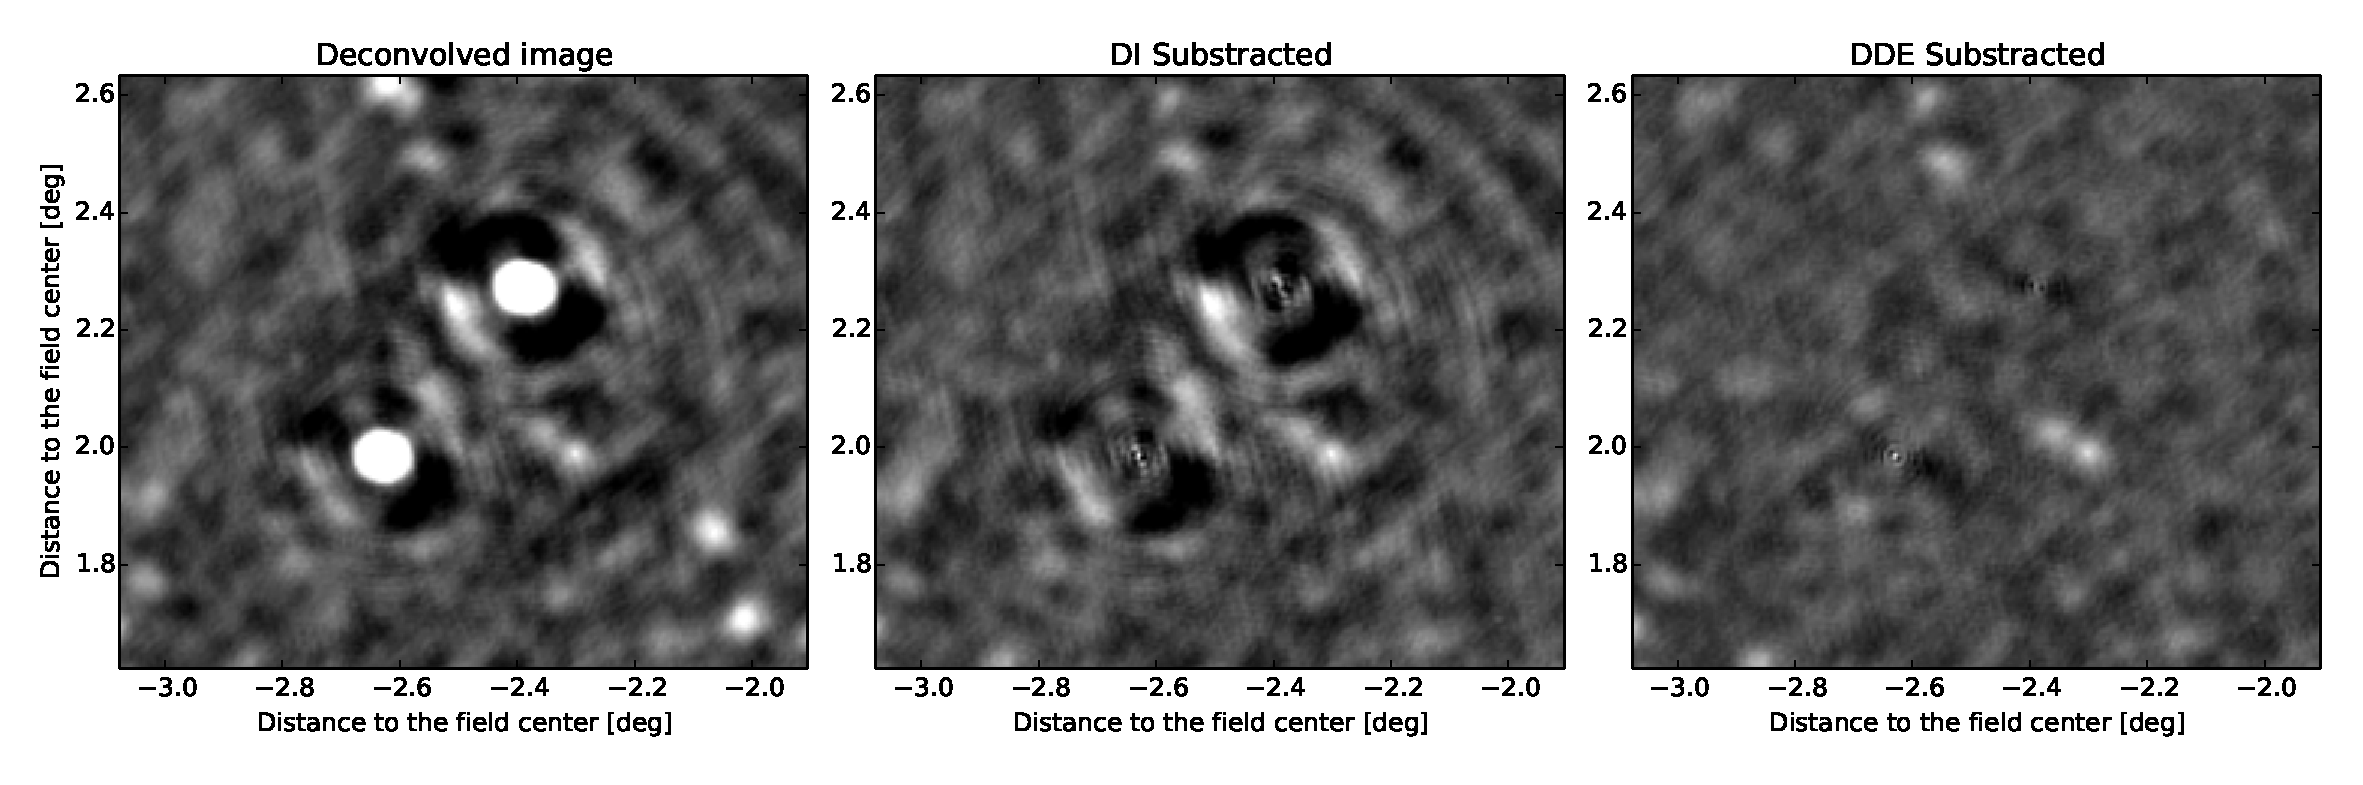
\includegraphics[width=17cm]{residZoom}
%% \caption{\label{fig:resid} This figure shows compares the image
%%   (left), the residuals data after simple skymodel substraction
%%   (center), and the residuals data after substracting the
%%   sky model corrupted by the direction-dependent solution (right).}
%% \end{center}
%% \end{figure*}



%===============================
\section{Iterative direction-dependent solver}

\subsection{Linear system for calibration}

If we write the
direction dependent gain vector as $\vec{g}$, which $i^{th}$ component
$i=d+a.n_d$ if the gain of antenna $a$ in direction $d$, then we find
the remarquable property that around the solution, Eq. \ref{eq:ME}
behaves like a linear system. Specifically, from Eq. \ref{eq:Jpq} and
\ref{eq:J}, it is easy to check that:

\begin{alignat}{2}
\label{eq:Lin}
\mathbf{v}=\left(\JV\big|_{\vec{g}}\right).\vec{g}
\end{alignat}

\noindent where $\JV\big|_{\vec{g}}$ mean that the Jacobian is
evaluated at $\vec{g}$.

Assuming a linear operator satisfying
Eq. \ref{eq:Lin} is given, we can build an iterative scheme to
derive an estimate $\widehat{\vec{g}}$ of $\vec{g}$. The linear operator
$\JV\big|_{\widehat{\vec{g}_i}}$ is build from the estimate
$\widehat{\vec{g}_i}$ at step $i$. Then Eq. \ref{eq:Lin} is solved
using the least-squares solution given by computing pseudo-inverse as follows:

\def\A{\textbf{A}}

\begin{alignat}{2}
\label{eq:Solve}
\widehat{\vec{g}_{i+1}}=&\left[\A^H\textbf{C}^{-1}\A\right]^{-1}\A^H\textbf{C}^{-1}\mathbf{v}\\
\label{eq:SolveA}
\text{with } \A=&\JV\big|_{\widehat{\vec{g}_i}}
\end{alignat}

\noindent where \textbf{C} is the covariance matrix of $\mathbf{v}$.


\subsection{Convergence and averaging}

As shown in Fig. ... the convergence of this algorithm is slow, and
following Stef-the-great, instead of estimating $\JV$ at
$\widehat{\vec{g}_i}$, we build it at a modified location constructed
from previous iterations, and Eq. \ref{eq:SolveA} becomes:

\begin{alignat}{2}
\A=&\JV\big|_{\widetilde{\vec{g}_i}}\\
\text{with } \widetilde{\vec{g}_i}=&(\widehat{\vec{g}_{i-1}}+\widehat{\vec{g}_{i}})/2
\end{alignat}




%% %===============================
%% \section{Connection with other existing algorithms}
\label{sec:Connection}

In this section, we investigate the connections between the complex
optimisation point of view (see Sec. \ref{sec:Wirtinger} and
\ref{sec:Solver}) and the existing algorithm. We show that antenna
based calibration schemes are always obtainable using this framework,
while general pealing based approaches are appliable under certain condition
of orthogonality between Fourier kernels.


\subsection{Levenberg-Maquardt and pealing}

\subsection{\sc{StefCal}}




%===============================


In this section, \COH\ is tested on simulated data for scalar Jones
matrices only. In Sec. \ref{sec:SimpleSimul}, the
Jones matrices are constant in time. In that case only the convergence
of \COH\ can be studied. In Sec. \ref{sec:VarSimul}, the Jones matrices vary in
time.

\begin{figure}
\begin{center}
\includegraphics[width=\columnwidth]{\FigDir Tessel.pdf}
\caption{\label{fig:tessel} In order to conduct direction-dependent
  calibration, the sources of the sky model are clustered using a Voronoi
  tessellation algorithm.}
\end{center}
\end{figure}

\subsubsection{Time-constant Jones matrices}
\label{sec:SimpleSimul}

For this test, a visibility dataset is simulated assuming the Low Frequency Array (LOFAR) antenna
layout. The phase center is located at
$(\alpha,\delta)=(14^h11^m20.5^s, +52^{o}12\arcmin10.0\arcsec)$,
the observing frequency is set $50$ MHz, and time
bins are 10 sec wide. To generate the visibilities, we use a sky model containing five
sources, distributed in a cross, and separated by a degree. The gains
applied to the antenna $p$ in direction $d$ are
constant through time, and are taken at random along a normal distribution
$g^{(d)}_{p}\sim\mathcal{N}\left(0,1\right)+i\mathcal{N}\left(0,1\right)$. The
data vector is then built from all baselines, and a $20$ minutes time chunk.

The corresponding matrix $(\JHJ)_\UL$ is shown in
Fig. \ref{fig:HalfJHJ}. It is block diagonal, each block having size
$\Nd\times\Nd$. The calibration solution convergence are shown
in Fig. \ref{fig:Convergence}. It is important to note that the
problems becomes better conditioned as the blocks of $(\JHJ)_\UL$
become more diagonally-dominated. In that case \COH\ converges faster, 
and this happens (i) when more data are taken into
account in the construction of the data vector or (ii) if the
directions are put further away from each other.

\subsubsection{Variable gains}
\label{sec:VarSimul}

In order to simulate a more realistic dataset, we use a 100 sources
sky model which flux density is randomly distributed (uniform
distribution). Noise is added to the visibilities at the $1\%$ level
of the total flux. The scalar Jones matrices are simulated assuming an
ionospheric model consisting of a purely scalar, direction-dependent
phase (an infinitesimally thin layer at a height of 100 km). The total
electron content (TEC) values at a set of sample points are generated
using Karhunen-Loeve decomposition \citep[the spatial correlation is
  given by Kolmogorov turbulence, see][]{Tol09}. The sources are
clustered in 10 directions using Voronoi tesselation
(Fig. \ref{fig:tessel}).

Fig. \ref{fig:resid} shows the residuals data computed by subtracting
the model data in the visibility domain, and the model data affected
by DDEs. The residual data standard deviation reduces by a factor
$\sim30$ after \COH~ has been applied.



%% \begin{figure*}
%% \begin{center}
%% %\hspace*{-1.3cm}
%% \includegraphics[width=\textwidth]{resid}
%% 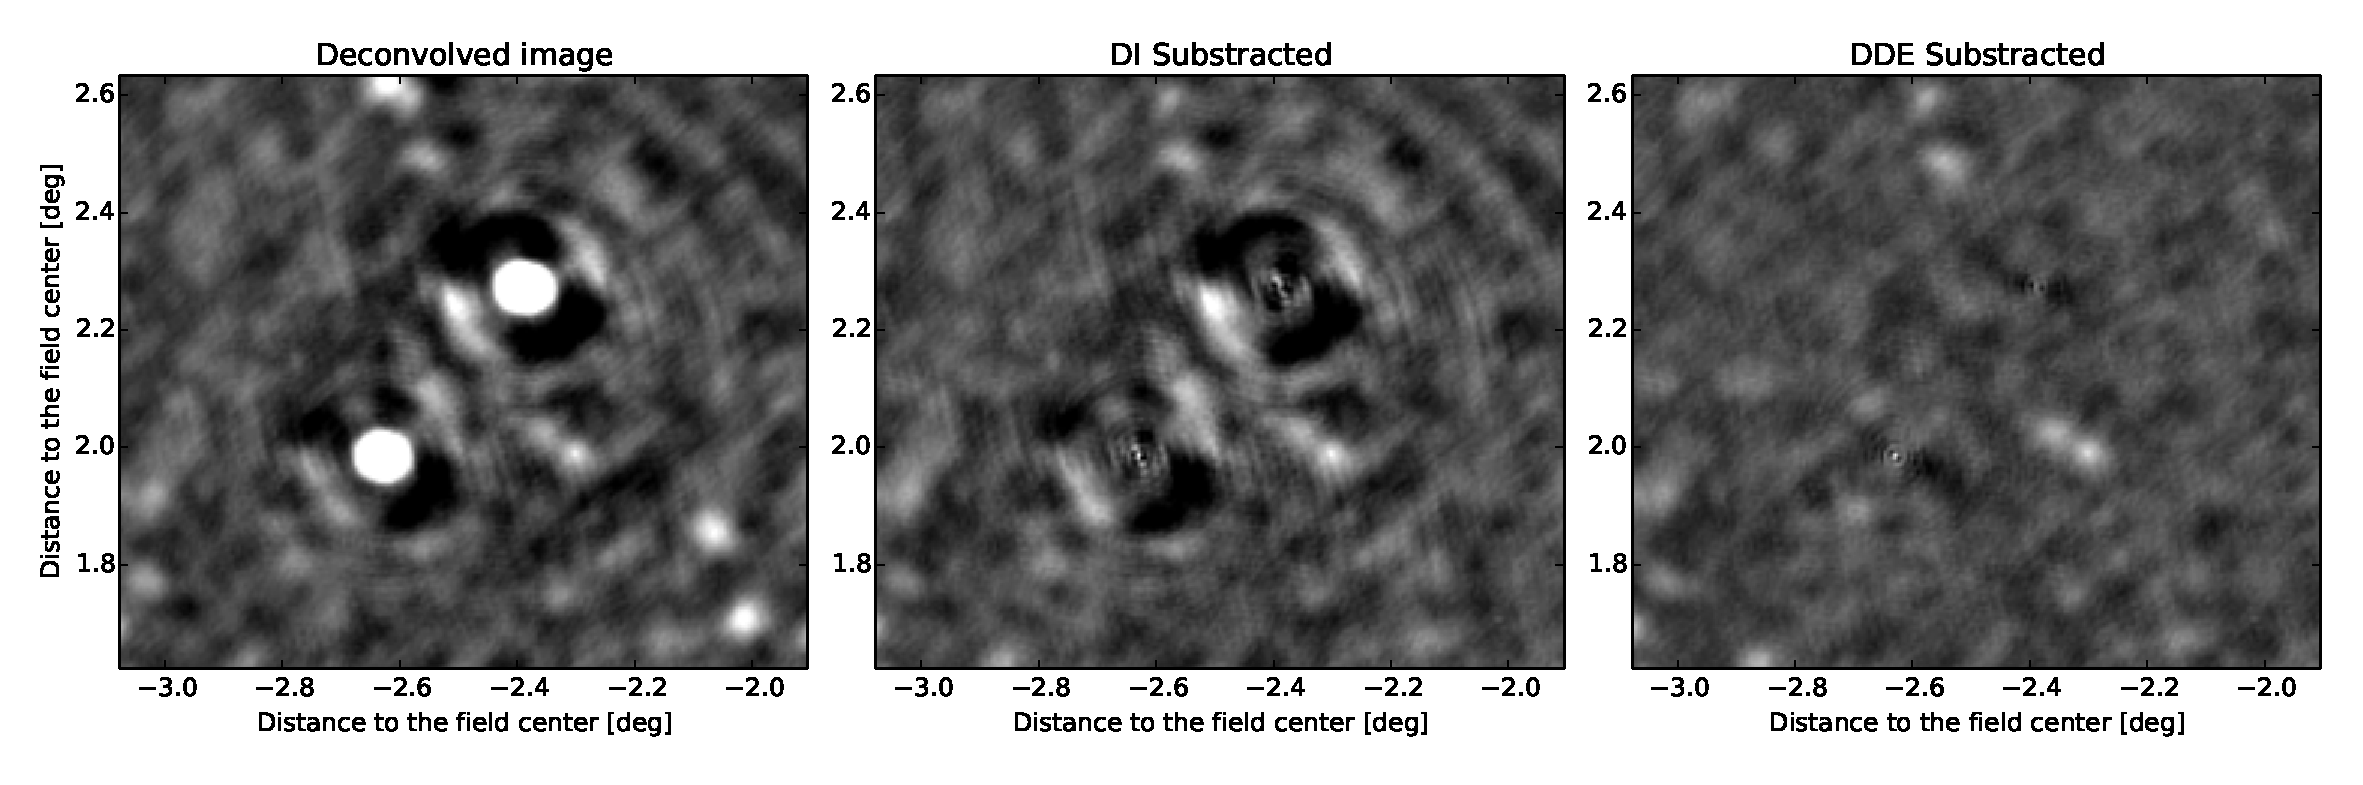
\includegraphics[width=\textwidth]{residZoom}
%% \caption{\label{fig:resid} This figure shows compares the image
%%   (left), the residuals data after simple skymodel substraction
%%   (center), and the residuals data after substracting the
%%   sky model corrupted by the direction-dependent solution (right).}
%% \end{center}
%% \end{figure*}



%===============================
\section{Conclusion}

This paper has presented a Levenberg-Maquardt based algorithm that
uses the Wirtinger's framework for complex derivative. The Jacobian
harbors a different structure that is sparser than in the classical
case. Based on this, a new optimisation algorithm has been
presented (\COH).

This framework, and its connection with existing algorithms will be
further discussed in \citet[][in prep.]{SmirnovTasse14}.






%% \begin{acknowledgements}
%% No thanks
%% \end{acknowledgements}


\bibliographystyle{aa}
\bibliography{references}

%\pagebreak
%\newpage


%% \begin{appendix}
%% \input{Initialisation.tex}
%% \input{NoiseProps.tex}
%% \end{appendix}

\end{document}



